\chapter{Metodologia}
\label{cap:metodologia}

\section{Ambiente de Simulação}
\label{sec:ambiente_simulacao}

O ambiente de simulação utilizado neste trabalho é o \textit{RL-SSL-EL}\footnote{\url{https://github.com/Werikcyano/RL-SSL-EL}} na versão de implementação da equipe de robótica Pequi Mecânico, conforme ilustrado na Figura \ref{fig:campo_simulacao}. \textit{RL-SSL-EL} é uma plataforma de simulação específica para o futebol de robôs na categoria \textit{Small Size League - Entry League (SSL-EL)}. Esta plataforma foi projetada para simplificar o processo de aprendizado por reforço aplicado ao futebol de robôs, oferecendo uma abstração adequada dos desafios físicos e técnicos básicos que são inerentes a este domínio.

\begin{figure}[h]
    \centering
    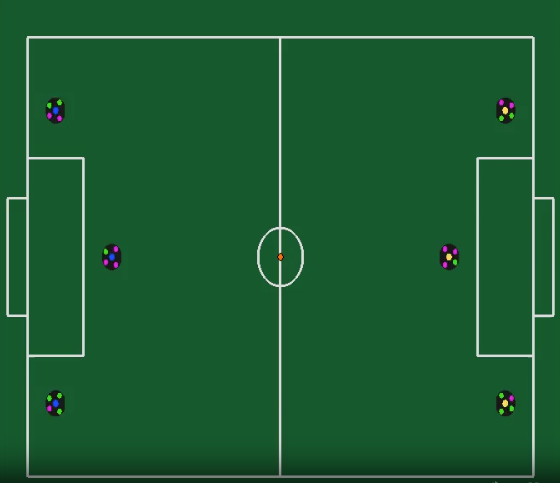
\includegraphics[width=0.8\textwidth]{fig/campo}
    \caption{Visualização do ambiente de simulação \textit{RL-SSL-EL} mostrando o campo de jogo com os robôs e a bola}
    \label{fig:campo_simulacao}
\end{figure}

\subsection{Características e Limitações}

O ambiente \textit{RL-SSL-EL} utiliza a biblioteca \textit{RLlib} para implementação dos algoritmos de aprendizado por reforço, o que permite a aplicação de técnicas como \textit{Proximal Policy Optimization (PPO)} de forma distribuída e eficiente. A simulação opera com base no modelo físico do futebol de robôs, incluindo movimentação dos robôs, dinâmica da bola, e interações entre os agentes no campo.

Entre as principais características do ambiente, destacam-se:

\begin{itemize}
    \item Compatibilidade com o \textit{framework RLlib} para treinamento distribuído;
    \item Suporte a múltiplos agentes na arquitetura multiagente;
    \item Sistema de recompensas configurável;
    \item Métricas de avaliação em tempo real;
    \item Capacidade de visualização do ambiente durante o treinamento.
\end{itemize}

As limitações mais relevantes incluem a simplificação dos aspectos físicos da simulação em comparação com ambientes mais complexos, e restrições nas estratégias de posicionamento dos robôs. Estas limitações, embora relevantes, não comprometem significativamente os objetivos deste trabalho, que foca principalmente na avaliação da eficácia do \textit{curriculum learning} em comparação com a abordagem \textit{self-play} convencional.

\subsection{Configurações Utilizadas}

O ambiente foi configurado para reproduzir um cenário de jogo simplificado, com parâmetros adequados para o treinamento efetivo dos agentes. As principais configurações incluem:

\begin{itemize}
    \item Frequência de atualização: 30 \textit{FPS} (\textit{frames} por segundo);
    \item Duração dos episódios: 40 segundos de jogo simulado;
    \item Número de agentes por equipe: 3 robôs (configurável conforme o estágio do \textit{curriculum});
    \item Posicionamento inicial: configurável para cada agente e para a bola;
    \item Limite de passos por episódio: variável conforme o estágio do \textit{curriculum} (300 a 500 passos)
\end{itemize}

Estas configurações foram ajustadas para oferecer um equilíbrio entre complexidade suficiente para o aprendizado significativo e simplicidade necessária para viabilizar o treinamento eficiente.

\section{Arquitetura do Sistema}
\label{sec:arquitetura_sistema}

\subsection{Modelo Base (\textit{Self-play Default})}

O sistema base utiliza a abordagem \textit{self-play} para treinamento dos agentes de futebol de robôs. Nesta abordagem, uma única política é treinada e utilizada tanto para os robôs da equipe azul (agentes em treinamento) quanto para a equipe amarela (oponentes). Esta configuração permite que os agentes evoluam continuamente, enfrentando versões cada vez mais competentes de si mesmos.

A arquitetura do sistema \textit{self-play} é implementada na classe \texttt{SelfPlayUpdateCallback}, responsável por gerenciar a atualização dos pesos da política dos oponentes. O funcionamento básico deste sistema segue os seguintes princípios:

\begin{enumerate}
    \item Uma política neural é treinada para os agentes da equipe azul;
    \item Uma cópia desta política é periodicamente transferida para os agentes da equipe amarela;
    \item A atualização ocorre quando a política azul atinge um nível de desempenho superior predefinido;
    \item A métrica utilizada para decidir sobre a atualização é baseada na diferença de pontuação entre as equipes
\end{enumerate}

Este processo cria um ciclo virtuoso de melhoria contínua, onde os agentes constantemente enfrentam oponentes que representam desafios adequados ao seu nível de habilidade atual.

\subsection{Adaptações Propostas por Este Trabalho}

Este trabalho propõe uma adaptação significativa ao sistema base, com a introdução do \textit{curriculum learning} como uma fase preparatória para o \textit{self-play}. Esta modificação visa estabelecer uma progressão mais estruturada no aprendizado dos agentes, permitindo que eles desenvolvam habilidades fundamentais antes de serem expostos aos desafios completos do futebol de robôs competitivo.

As principais adaptações incluem:

\begin{enumerate}
    \item Implementação da classe \texttt{SSLCurriculumEnv}, que estende a classe base \texttt{SSLMultiAgentEnv} para suportar diferentes níveis de complexidade no treinamento;
    
    \item Desenvolvimento do \texttt{CurriculumCallback}, responsável por monitorar o desempenho dos agentes e controlar a progressão entre os níveis do \textit{curriculum};
    
    \item Criação de um sistema de configuração modular para os diferentes estágios do \textit{curriculum}, permitindo ajustes precisos nos parâmetros de cada nível;
    
    \item Implementação de métricas específicas para avaliar o desempenho dos agentes em cada estágio do \textit{curriculum}.
\end{enumerate}

Estas adaptações permitem uma transição suave do treinamento estruturado para o ambiente competitivo, potencialmente melhorando a eficiência do aprendizado e a qualidade das políticas resultantes.

\subsection{Pipeline de Treinamento}

O \textit{pipeline} de treinamento implementado neste trabalho integra o \textit{curriculum learning} e o \textit{self-play} em uma sequência coerente, permitindo que os agentes progridam de forma gradual de tarefas simples até o jogo completo. A Figura \ref{fig:fluxograma_treino} apresenta uma visão geral deste processo, ilustrando a estrutura do \textit{pipeline} e a interação entre seus componentes.

\begin{figure}[H]
    \centering
    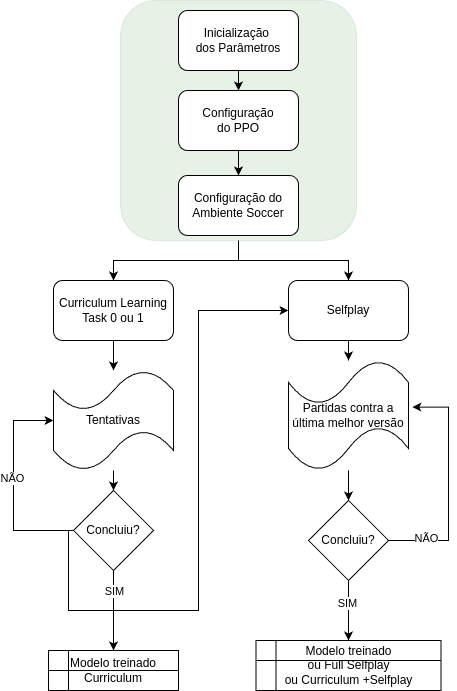
\includegraphics[width=0.85\textwidth]{fig/fluxograma_treino_mestrado.png}
    \caption{Fluxograma do \textit{pipeline} de treinamento, destacando a integração entre \textit{Curriculum Learning} e \textit{Self-play}. O processo inicia com a inicialização e configuração dos componentes, seguido pela divisão entre as abordagens de \textit{Curriculum Learning} e \textit{Self-play} direto. A fase de \textit{Curriculum Learning} inclui tarefas progressivas (\textit{Task} 0 ou 1) seguidas por ciclos de tentativas até conclusão do critério de promoção, resultando em um modelo treinado que serve como base para o \textit{Self-play} subsequente. Fonte: Elaborado pelo autor.}
    \label{fig:fluxograma_treino}
\end{figure}

Como ilustrado no fluxograma, este \textit{pipeline} é composto por três estágios principais:

\begin{enumerate}
    \item \textbf{Treinamento com \textit{Curriculum Learning}}: Os agentes iniciam o treinamento em um ambiente simplificado, com tarefas específicas de complexidade progressiva (\textit{Task} 0 ou 1). Este estágio utiliza o \texttt{CurriculumCallback} para monitorar o desempenho e controlar a progressão através de ciclos de tentativas até que os critérios de conclusão sejam atingidos.
    
    \item \textbf{Transição para \textit{Self-play}}: Após completar os estágios do \textit{curriculum}, os agentes são transferidos para o ambiente de \textit{self-play}, onde enfrentam versões anteriores de si mesmos como oponentes.
    
    \item \textbf{Refinamento com \textit{Self-play}}: Os agentes continuam o treinamento no ambiente competitivo, com atualizações periódicas da política dos oponentes quando alcançam níveis de desempenho predefinidos, através de partidas contra a última melhor versão.
\end{enumerate}

A implementação deste processo de treinamento é feita através de um arquivo central que organiza e coordena todas as etapas necessárias. Este arquivo é responsável por configurar o ambiente de treinamento e definir como os robôs devem se comportar em cada fase. A mudança entre as diferentes fases do treinamento pode ser facilmente ajustada através de configurações específicas, permitindo maior flexibilidade durante todo o processo.

\section{Implementação do \textit{Curriculum Learning}}
\label{sec:implementacao_cl}

\subsection{Visão Geral da Arquitetura do \textit{Curriculum}}

A arquitetura do \textit{curriculum learning} implementada neste trabalho segue uma estrutura de estágios progressivos, onde cada estágio representa um nível de complexidade específico no aprendizado do futebol de robôs. A progressão entre estes estágios é controlada por critérios de desempenho predefinidos, garantindo que os agentes desenvolvam as habilidades necessárias antes de avançar para desafios mais complexos.

A transição do cenário curricular é projetada para preservar a continuidade do aprendizado, evitando mudanças abruptas que poderiam prejudicar o desenvolvimento dos agentes. Esta arquitetura foi inspirada em sistemas de treinamento progressivo observados em jogos eletrônicos populares, como FIFA e \textit{Rocket League}, onde os jogadores são introduzidos gradualmente a conceitos mais complexos.

\begin{figure}[H]
    \centering
    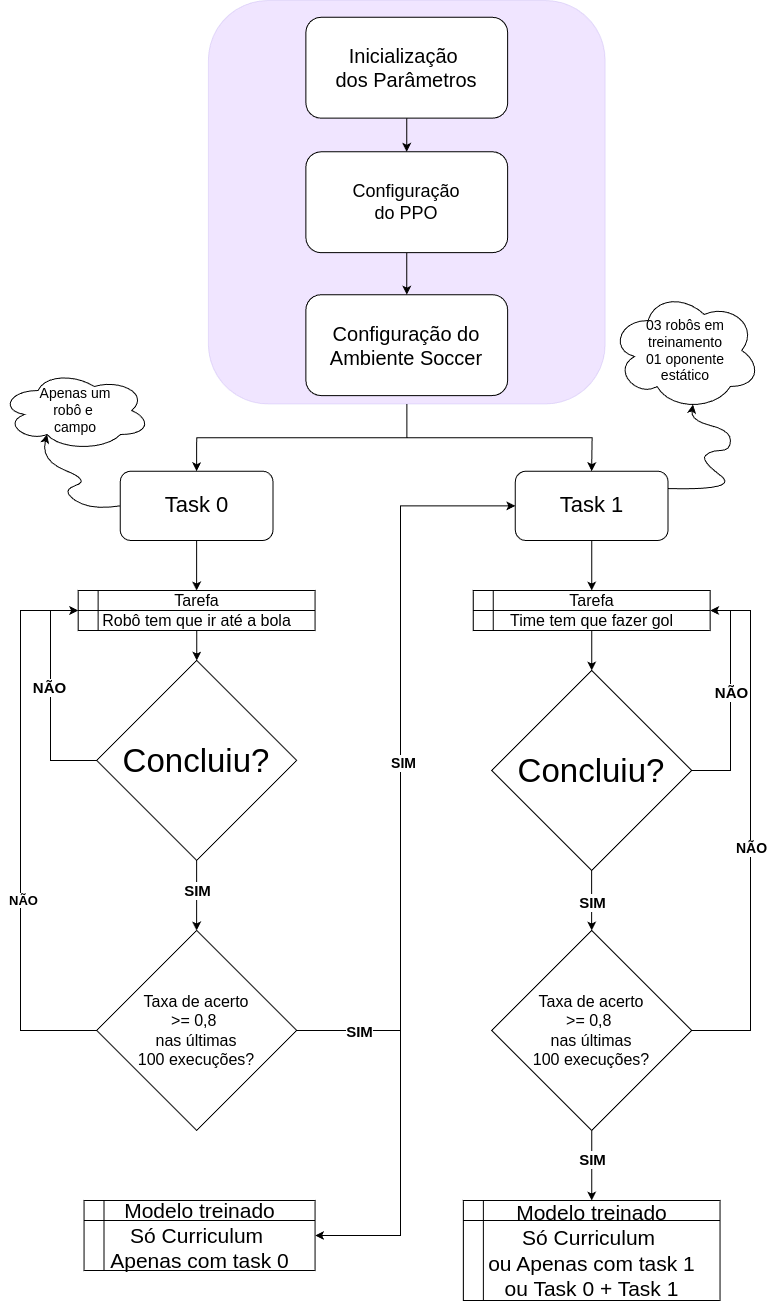
\includegraphics[width=0.85\textwidth]{fig/fluxograma_treino_curriculum.png}
    \caption{Diagrama de fluxo do processo de treinamento com \textit{curriculum learning}. Fonte: Elaborado pelo autor.}
    \label{fig:diagrama_curriculum}
\end{figure}

O fluxo do processo inicia com a definição dos estágios e seus respectivos parâmetros no arquivo de configuração \texttt{config.yaml}. Estes parâmetros incluem critérios de sucesso, sistemas de recompensa específicos, e configurações do ambiente para cada estágio. Durante o treinamento, o \texttt{CurriculumCallback} monitora continuamente o desempenho dos agentes, calculando a taxa de sucesso com base em uma janela deslizante de episódios recentes. Quando esta taxa atinge o limiar de promoção predefinido, o sistema avança automaticamente para o próximo estágio do \textit{curriculum}.

\subsection{Estrutura dos Estágios}

O \textit{curriculum} implementado neste trabalho é estruturado em três estágios principais, cada um representando um nível distinto de complexidade no aprendizado do futebol de robôs. Estes estágios são designados como tarefas (\textit{tasks}) e numerados de 0 a 1, com cada tarefa apresentando configurações e objetivos específicos.

\subsubsection{Estágio 1 (\textit{Task} 0): Fundamentos Básicos}
\label{subsubsec:estagio1}

O Estágio 1 representa o nível mais básico do \textit{curriculum}, focado no desenvolvimento de habilidades fundamentais sem a presença de oponentes. Neste estágio, os agentes aprendem a se aproximar e interagir com a bola em um ambiente controlado.

\paragraph{Configuração do Ambiente}

No Estágio 1, o ambiente é configurado com as seguintes características:
\begin{itemize}
    \item Um robô da equipe azul, posicionado em local predefinido;
    \item Ausência de robôs oponentes (equipe amarela);
    \item Bola posicionada no centro do campo;
    \item Limite de 300 passos por episódio.
\end{itemize}

\paragraph{Sistema de Recompensas}

O sistema de recompensas para este estágio é simplificado, focando primariamente no contato com a bola. A estrutura de recompensas inclui:
\begin{itemize}
    \item Recompensa principal (10 pontos) concedida quando um agente toca na bola;
    \item Recompensas incrementais relacionadas à aproximação da bola;
    \item Penalidades por tempo excessivo sem interação com a bola.
\end{itemize}

\paragraph{Critérios de Progressão}

Para avançar deste estágio para o próximo, os agentes devem demonstrar consistência em sua capacidade de interagir com a bola. Especificamente:
\begin{itemize}
    \item Taxa de sucesso de pelo menos 80\% em uma janela de 100 episódios;
    \item O sucesso é definido como tocar na bola pelo menos uma vez durante o episódio.
\end{itemize}

\subsubsection{Estágio 2 (\textit{Task} 1): Interação com Oponentes Estáticos}
\label{subsubsec:estagio2}

O Estágio 2 introduz um nível intermediário de complexidade, apresentando oponentes estáticos e objetivos táticos mais elaborados. Neste estágio, os agentes precisam aprender a navegar em um ambiente com obstáculos e realizar ações mais coordenadas.

\paragraph{Configuração do Ambiente}

O ambiente neste estágio apresenta as seguintes características:
\begin{itemize}
    \item Três robôs da equipe azul, mantendo a formação básica com pequena variação nas posições;
    \item Um robô oponente (equipe amarela), posicionado estrategicamente próximo à bola;
    \item Bola posicionada no centro, com variações aleatórias limitadas;
    \item Limite de 400 passos por episódio.
\end{itemize}

\paragraph{Sistema de Recompensas}

O sistema de recompensas é expandido para incluir objetivos táticos mais avançados:
\begin{itemize}
    \item Recompensa por proximidade à bola (10\% do peso total);
    \item Recompensa por conduzir a bola em direção ao gol adversário (30\% do peso);
    \item Recompensa substancial por marcar gols (10 pontos);
    \item Recompensa menor por manter posse de bola (5\% do peso).
\end{itemize}

\paragraph{Critérios de Progressão}

A progressão para o próximo estágio requer habilidades táticas mais avançadas:
\begin{itemize}
    \item Taxa de sucesso de pelo menos 80\% em uma janela de 100 episódios;
    \item O sucesso neste estágio é definido como marcar pelo menos um gol durante o episódio.
\end{itemize}

%\subsubsection{Estágio 3 (\textit{Task} 2): Jogo Completo com Oponentes Ativos}
%\label{subsubsec:estagio3}

%O Estágio 3 representa o nível mais avançado do \textit{curriculum}, introduzindo múltiplos oponentes ativos e aproximando-se das condições reais de jogo. Neste estágio, os agentes precisam demonstrar capacidades táticas complexas e coordenação de equipe.

%\paragraph{Configuração do Ambiente}

%O ambiente neste estágio apresenta complexidade máxima:
%\begin{itemize}
%    \item Três robôs da equipe azul, com posicionamento tático
%    \item Três robôs oponentes (equipe amarela), distribuídos estrategicamente pelo campo
%    \item Posições iniciais configuradas para simular situações táticas realistas
%    \item Limite de 500 passos por episódio
%\end{itemize}

%\paragraph{Sistema de Recompensas}

%O sistema de recompensas é refinado para valorizar aspectos estratégicos do jogo:
%\begin{itemize}
%    \item Manutenção das recompensas por proximidade à bola e ao gol
%    \item Valorização adicional de comportamentos defensivos quando necessário
%    \item Penalizações por violações das regras (saída da bola, faltas)
%    \item Recompensas por posicionamento tático eficiente
%\end{itemize}

\paragraph{Transição para \textit{Self-play}}

Após completar este estágio, os agentes são considerados preparados para o treinamento \textit{self-play}, onde enfrentarão versões cada vez mais competentes de si mesmos. Esta transição marca a conclusão do \textit{curriculum} estruturado e o início da fase competitiva do treinamento.

\subsection{Mecanismo de Transição entre Estágios}
\label{subsec:mecanismo_transicao}

O mecanismo de transição entre os estágios do \textit{curriculum} é implementado na classe \texttt{CurriculumCallback}, responsável por monitorar o desempenho dos agentes e decidir sobre a progressão para o próximo nível. Este mecanismo opera com base em critérios objetivos de desempenho, garantindo que os agentes desenvolvam as habilidades necessárias antes de enfrentar desafios mais complexos.

\subsubsection{Monitoramento de Desempenho}

O monitoramento de desempenho é realizado através de um conjunto de métricas coletadas durante o treinamento. Para cada episódio, o sistema registra:

\begin{itemize}
    \item Indicadores de sucesso específicos para o estágio atual (toque na bola, gols marcados);
    \item Tempo necessário para concluir as tarefas;
    \item Eficiência das trajetórias e ações;
    \item Métricas de continuidade (\textit{resets}).
\end{itemize}

Estas métricas são armazenadas em uma janela deslizante de episódios recentes, permitindo a avaliação do desempenho atual com base em um histórico significativo. A implementação utiliza a estrutura \texttt{deque} do \textit{Python} para manter esta janela de forma eficiente, com um tamanho configurável (padrão de 100 episódios).

\subsubsection{Adaptação Dinâmica}

Quando a taxa de sucesso calculada sobre a janela de episódios atinge o limiar de promoção (configurado como 80\% no sistema atual), o mecanismo de transição executa as seguintes ações:

\begin{enumerate}
    \item Incrementa o nível da tarefa atual (\texttt{task\_level});
    \item Atualiza esta mudança em todos os ambientes paralelos em execução;
    \item Reseta as estatísticas de desempenho para o novo estágio;
    \item Ajusta os parâmetros do ambiente conforme as especificações do próximo estágio.
\end{enumerate}

Esta transição é realizada de forma sincronizada em todos os ambientes, garantindo consistência no processo de treinamento distribuído. O sistema também registra informações detalhadas sobre cada transição, permitindo análises posteriores sobre a progressão do aprendizado.

\subsection{Integração com \textit{Self-play}}
\label{subsec:integracao_selfplay}

A integração entre o \textit{curriculum learning} e o \textit{self-play} representa um aspecto fundamental da abordagem proposta neste trabalho. Esta integração permite uma transição suave do treinamento estruturado para o ambiente competitivo, combinando os benefícios de ambas as abordagens.

\subsubsection{Transição para Treinamento Competitivo}

A transição do \textit{curriculum learning} para o \textit{self-play} ocorre após a conclusão do último estágio do \textit{curriculum} (\textit{Task} 2). Neste ponto, os agentes da equipe azul já desenvolveram as habilidades fundamentais necessárias para o jogo e estão preparados para enfrentar oponentes mais desafiadores.

O processo de transição segue os seguintes passos:

\begin{enumerate}
    \item Os pesos da política treinada com \textit{curriculum} são preservados;
    \item O ambiente é reconfigurado para o modo \textit{self-play} completo;
    \item A política da equipe amarela é inicializada com os mesmos pesos da equipe azul;
    \item O mecanismo de atualização da equipe amarela é ativado.
\end{enumerate}

Esta abordagem permite que os agentes continuem seu desenvolvimento a partir do ponto alcançado com o \textit{curriculum}, sem perder o progresso já realizado. A transição é implementada no arquivo \texttt{rllib\_multiagent.py}, que gerencia a configuração geral do treinamento.

\subsubsection{Métricas de Acompanhamento}

Para avaliar a eficácia da integração entre \textit{curriculum learning} e \textit{self-play}, são monitoradas diversas métricas durante a fase de transição e o subsequente treinamento competitivo. As principais métricas incluem:

\begin{itemize}
    \item Taxa de vitória da equipe azul contra a equipe amarela;
    \item Tempo médio dos episódios;
    \item Métricas de continuidade do jogo (\textit{resets}).
\end{itemize}

Estas métricas permitem uma avaliação objetiva do impacto do \textit{curriculum learning} sobre o desempenho dos agentes no ambiente competitivo, fornecendo insights sobre os benefícios potenciais desta abordagem em comparação com o \textit{self-play} puro.

\subsection{Implementação Técnica}
\label{subsec:implementacao_tecnica}

A implementação técnica do \textit{curriculum learning} neste trabalho envolve diversos componentes interconectados, cada um responsável por aspectos específicos do processo de treinamento. Esta seção detalha as estruturas de dados e parâmetros de configuração utilizados na implementação.

\subsubsection{Estruturas de Dados}

As principais estruturas de dados utilizadas na implementação incluem:

\begin{itemize}
    \item \texttt{SSLCurriculumEnv}: Classe principal que estende o ambiente base para suportar os diferentes estágios do \textit{curriculum}. Esta classe mantém estado interno sobre o nível atual da tarefa, métricas de desempenho, e configurações específicas de cada estágio.
    
    \item \texttt{CurriculumCallback}: Classe responsável pelo monitoramento do desempenho e controle da progressão entre estágios. Utiliza estruturas como \texttt{deque} para manter históricos de desempenho e métricas estatísticas.
    
    \item \texttt{ConfigDict}: Estrutura hierárquica que armazena os parâmetros de configuração para cada estágio do \textit{curriculum}, incluindo configurações do ambiente, sistema de recompensas, e critérios de sucesso.
    
    \item \texttt{ContinuityMetrics}: Estrutura para armazenar métricas relacionadas à continuidade do jogo, como número de \textit{resets}.
\end{itemize}

Estas estruturas são implementadas utilizando classes e dicionários do \textit{Python}, com suporte para serialização e desserialização através da biblioteca \textit{YAML}, facilitando a configuração e o ajuste dos parâmetros do treinamento.

%\subsubsection{Parâmetros de Configuração}

%Os parâmetros de configuração do \textit{curriculum} são definidos no arquivo \texttt{config.yaml}, utilizando uma estrutura hierárquica que permite especificar detalhadamente as características de cada estágio. Os principais parâmetros incluem:

%\begin{itemize}
%    \item \texttt{enabled}: Flag para ativar ou desativar o \textit{curriculum learning}
%    \item \texttt{initial\_task}: Estágio inicial do \textit{curriculum} (0, 1, ou 2)
%    \item \texttt{promotion\_threshold}: Taxa de sucesso necessária para avançar para o próximo estágio (padrão: 0.8)
%    \item \texttt{evaluation\_window}: Número de episódios para avaliar o desempenho (padrão: 100)
%    \item \texttt{tasks}: Dicionário contendo as configurações específicas de cada estágio:
%    \begin{itemize}
%        \item \texttt{max\_steps}: Limite de passos por episódio
%        \item \texttt{num\_agents\_blue} e \texttt{num\_agents\_yellow}: Número de agentes em cada equipe
%        \item \texttt{init\_pos}: Posições iniciais dos robôs e da bola
%        \item \texttt{reward\_weights}: Pesos das diferentes componentes da recompensa
%        \item \texttt{success\_criteria}: Critérios para considerar um episódio bem-sucedido
%    \end{itemize}
%\end{itemize}

%Esta estrutura de configuração oferece grande flexibilidade para ajustar o \textit{curriculum} de acordo com necessidades específicas, permitindo experimentação com diferentes progressões de aprendizado.

\section{Métricas de Avaliação}
\label{sec:metricas_avaliacao}

Para avaliar o desempenho dos agentes e comparar a eficácia das abordagens de treinamento, foi desenvolvido um conjunto abrangente de métricas que captura diferentes aspectos do comportamento dos agentes. Estas métricas são coletadas durante o treinamento e utilizadas para análises comparativas.

%\subsection{Número de Gols}

%O número de gols marcados representa uma das métricas mais diretas de desempenho no futebol de robôs. Esta métrica é registrada tanto por episódio quanto de forma acumulada ao longo do treinamento, permitindo avaliar a evolução da capacidade ofensiva dos agentes. As submétrias relacionadas incluem:

%\begin{itemize}
%    \item Gols marcados por episódio
%    \item Gols sofridos por episódio
%    \item Percentual de episódios com pelo menos um gol
%    \item Diferença líquida de gols
%\end{itemize}

%Estas métricas fornecem insights sobre a eficácia ofensiva e defensiva dos agentes, aspectos fundamentais do desempenho no futebol de robôs.

\subsection{Tempo dos Episódios}

O tempo dos episódios é uma métrica importante para avaliar a eficiência do jogo e a capacidade dos agentes de alcançar seus objetivos rapidamente. Esta métrica é analisada em diferentes dimensões:

\begin{itemize}
    \item Duração média dos episódios (em passos);
    \item Evolução da duração ao longo do treinamento;
    \item Distribuição dos tempos de episódio.
\end{itemize}

Um aspecto particularmente relevante desta métrica é sua relação com a progressão do treinamento. Tipicamente, espera-se que episódios mais curtos indiquem agentes mais eficientes na realização de seus objetivos.

\subsection{Métrica de Continuidade}

As métricas de continuidade foram desenvolvidas especificamente para este trabalho, visando avaliar a fluidez do jogo e a capacidade dos agentes de manter a bola em jogo por períodos prolongados. Estas métricas incluem:

\begin{itemize}
    \item Número total de \textit{resets} durante todo o treinamento;
    \item Média de \textit{resets} por episódio.
\end{itemize}

Estas métricas são particularmente importantes para avaliar a qualidade do jogo produzido pelos agentes, uma vez que um jogo com menos interrupções tende a ser mais dinâmico e interessante.

%\subsection{Posse de Bola}

%A posse de bola é uma métrica táctica importante que reflete a capacidade dos agentes de controlar o jogo. Para esta análise, são considerados os seguintes aspectos:

%\begin{itemize}
%    \item Percentual de posse de bola por equipe
%    \item Duração média das sequências de posse
%    \item Correlação entre posse e resultados (gols)
%    \item Distribuição espacial da posse no campo
%\end{itemize}

%A análise desta métrica permite compreender as estratégias emergentes dos agentes e sua eficácia em diferentes contextos do jogo.

\subsection{Recompensa Acumulada}

A recompensa acumulada representa a métrica fundamental do aprendizado por reforço, refletindo diretamente o objetivo de otimização dos agentes. Esta métrica é analisada em várias dimensões:

\begin{itemize}
    \item Recompensa média por episódio;
    \item Evolução da recompensa ao longo do treinamento.
\end{itemize}

A análise da recompensa acumulada permite avaliar a convergência do treinamento e comparar diretamente diferentes abordagens em termos de sua eficácia em otimizar o comportamento dos agentes.

\subsection{Avaliação em Torneio}

Para uma avaliação mais abrangente e objetiva do desempenho dos modelos, será realizado um torneio competitivo entre o modelo \textit{baseline} (treinado com \textit{self-play} padrão) e o modelo proposto (incorporando \textit{curriculum learning}). Este torneio permitirá:

\begin{itemize}
    \item Comparação direta do desempenho em condições controladas;
    \item Avaliação da robustez das estratégias aprendidas;
    \item Análise da consistência dos resultados em múltiplas partidas;
    \item Identificação de possíveis vantagens táticas específicas.
\end{itemize}

O formato do torneio será estruturado para garantir uma avaliação estatisticamente significativa, com múltiplas partidas entre os modelos. Os resultados deste torneio fornecerão evidências importantes sobre a eficácia prática das modificações propostas no processo de treinamento.


Além das métricas específicas descritas anteriormente, também serão utilizadas algumas métricas padrão do aprendizado por reforço:

\begin{itemize}
    \item \textit{Entropy} - Mede a aleatoriedade das ações selecionadas pela política, indicando o nível de exploração do agente;
    \item \textit{Policy Loss} - Quantifica o erro na política atual em relação à política ótima estimada;
    \item \textit{VF Explained} - Indica quanto da variância nas recompensas é explicada pelo modelo de valor, medindo a qualidade das estimativas do valor
\end{itemize}


